\begin{enumerate}[label=\thesection.\arabic*.,ref=\thesection.\theenumi]
\numberwithin{equation}{enumi}

\item The Block diagram of a system is illustrated in the figure shown, where $X(s)$ is the input and $Y(s)$ is the output. Draw the equivalent signal flow graph.
\renewcommand{\thefigure}{\theenumi.\arabic{figure}}

\begin{figure}[!ht]
\centering
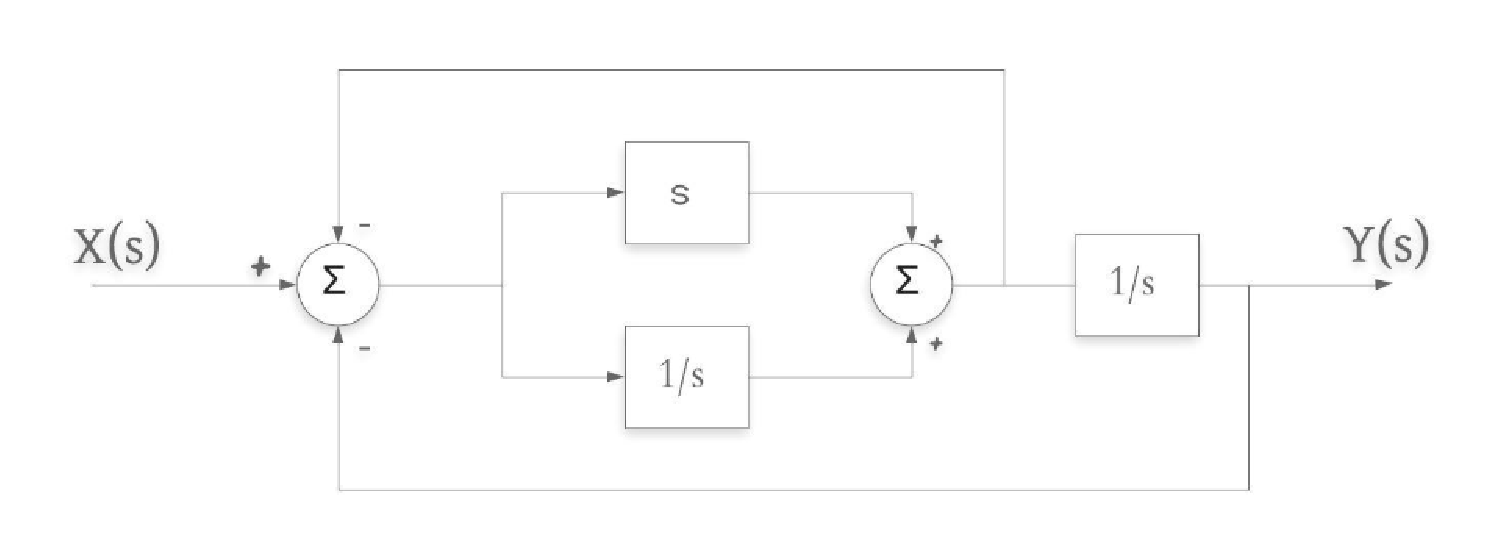
\includegraphics[width=\columnwidth]{./figs/pic1.eps}
\caption{}
\label{fig:sec_order}
\end{figure}
\solution
Signal flow graph of given above block diagram is
\begin{figure}[!ht]
\begin{tikzpicture}
[
label revd/.is if=labrev,
amark/.style={
            decoration={             
                        markings,   
                        mark=at position {0.5} with { 
                                    \arrow{stealth},
                                    \iflabrev \node[above] {#1};\else \node[below] {#1};\fi
                        }
            },
            postaction={decorate}
},
terminal/.style 2 args={draw,circle,inner sep=1pt,label={#1:#2}},
]

%Place the nodes
\node[terminal={below}{$X(s)$}] (a) at (0,0) {};
\node[terminal={below}{$N_1$}] (b) at (1cm,0) {};
\node[terminal={below}{$N_2$}] (c) at (2cm,0) {};
\node[terminal={[xshift=-4mm]below right}{$N_3$}] (d) at (5cm,0) {};
\node[terminal={below}{$N_4$}] (e) at (6cm,0) {};
\node[terminal={below}{$N_5$}] (f) at (7.8cm,0) {};
\node[terminal={below}{$Y(s)$}] (g) at (8.8cm,0) {};
%Draw the connections
\draw[amark=$ $] (a) to (b);
\draw[amark=$ $] (b) to (c);
\draw[amark=$s$] (c) to[bend left=45] (d);
\draw[amark=$1/s$] (e) to (f);
\draw[amark=$ $] (f) to (g);
\draw[amark=$ $] (d) to (e);
\draw[amark=$1/s$] (c) to[bend left=-45] (d);
\draw[amark=$-1$] (e) to[bend left=-60] (b);
\draw[amark=$-1$,label revd] (f) to[bend left=60] (b);
%\draw[amark=$-K/M$,label revd] (e) to[bend right=50] (c);
\end{tikzpicture}
\caption{signal flow graph}
\label{fig:sec_order}
\end{figure}
%
\renewcommand{\thefigure}{\theenumi}
\item Draw all the forward paths and compute the respective gains.
\renewcommand{\thefigure}{\theenumi.\arabic{figure}}
\solution
Here, 
\begin{align}
P_1=\frac{s}{s}=1
\end{align}

\begin{figure}[!ht]
\begin{tikzpicture}
[
label revd/.is if=labrev,
amark/.style={
            decoration={             
                        markings,   
                        mark=at position {0.5} with { 
                                    \arrow{stealth},
                                    \iflabrev \node[above] {#1};\else \node[below] {#1};\fi
                        }
            },
            postaction={decorate}
},
terminal/.style 2 args={draw,circle,inner sep=1pt,label={#1:#2}},
]

%Place the nodes
\node[terminal={below}{$X(s)$}] (a) at (0,0) {};
\node[terminal={below }{$N_1$}] (b) at (1cm,0) {};
\node[terminal={below }{$N_2$}] (c) at (2cm,0) {};
\node[terminal={[xshift=-4mm]below right}{$N_3$}] (d) at (4cm,0) {};
\node[terminal={below }{$N_4$}] (e) at (6cm,0) {};
\node[terminal={below }{$N_5$}] (f) at (8cm,0) {};
\node[terminal={below }{$Y(s)$}] (g) at (9.5cm,0) {};
%Draw the connections
\draw[amark=$ $] (a) to (b);
\draw[amark=$ $] (b) to (c);
\draw[amark=$s$] (c) to[bend left=45] (d);
\draw[amark=$1/s$] (e) to (f);
\draw[amark=$ $] (f) to (g);
\draw[amark=$ $] (d) to (e);
%\draw[amark=$1/s$] (c) to[bend left=-45] (d);
%\draw[amark=$-1$] (e) to[bend left=-45] (b);
%\draw[amark=$-1$,label revd] (f) to[bend left=50] (b);
%\draw[amark=$-K/M$,label revd] (e) to[bend right=50] (c);
\end{tikzpicture}
\caption{$P_1$}
\label{fig:sec_order}
\end{figure}

 
\begin{align}
P_2=(1/s)(1/s)=1/s^2
\end{align}

\begin{figure}[!ht]
\begin{tikzpicture}
[
label revd/.is if=labrev,
amark/.style={
            decoration={             
                        markings,   
                        mark=at position {0.5} with { 
                                    \arrow{stealth},
                                    \iflabrev \node[above] {#1};\else \node[below] {#1};\fi
                        }
            },
            postaction={decorate}
},
terminal/.style 2 args={draw,circle,inner sep=1pt,label={#1:#2}},
]

%Place the nodes
\node[terminal={below}{$X(s)$}] (a) at (0,0) {};
\node[terminal={below }{$N_1$}] (b) at (1cm,0) {};
\node[terminal={below }{$N_2$}] (c) at (2cm,0) {};
\node[terminal={[xshift=-4mm]below right}{$N_3$}] (d) at (4cm,0) {};
\node[terminal={below }{$N_4$}] (e) at (6cm,0) {};
\node[terminal={below }{$N_5$}] (f) at (8cm,0) {};
\node[terminal={below }{$Y(s)$}] (g) at (9.5cm,0) {};
%Draw the connections
\draw[amark=$ $] (a) to (b);
\draw[amark=$ $] (b) to (c);
%\draw[amark=$s$] (c) to[bend left=45] (d);
\draw[amark=$1/s$] (e) to (f);
\draw[amark=$ $] (f) to (g);
\draw[amark=$ $] (d) to (e);
\draw[amark=$1/s$] (c) to[bend left=-45] (d);
%\draw[amark=$-1$] (e) to[bend left=-45] (b);
%\draw[amark=$-1$,label revd] (f) to[bend left=50] (b);
%\draw[amark=$-K/M$,label revd] (e) to[bend right=50] (c);
\end{tikzpicture}
\caption{$P_2$}
\label{fig:sec_order}
\end{figure}
\renewcommand{\thefigure}{\theenumi}

\item Draw the loops and calculate the respective gains.\renewcommand{\thefigure}{\theenumi.\arabic{figure}}
\\
\solution 
\begin{align}
L_1=(-1)(s)=-s
\end{align}

\begin{figure}[!ht]
\begin{tikzpicture}
[
label revd/.is if=labrev,
amark/.style={
            decoration={             
                        markings,   
                        mark=at position {0.5} with { 
                                    \arrow{stealth},
                                    \iflabrev \node[above] {#1};\else \node[below] {#1};\fi
                        }
            },
            postaction={decorate}
},
terminal/.style 2 args={draw,circle,inner sep=1pt,label={#1:#2}},
]

%Place the nodes
%\node[terminal={below}{$X(s)$}] (a) at (0,0) {};
\node[terminal={below }{$N_1$}] (b) at (2cm,0) {};
\node[terminal={below }{$N_2$}] (c) at (4cm,0) {};
\node[terminal={[xshift=-4mm]below right}{$N_3$}] (d) at (6cm,0) {};
\node[terminal={below }{$N_4$}] (e) at (8cm,0) {};
%\node[terminal={below left}{$N_5$}] (f) at (11cm,0) {};
%\node[terminal={below left}{$Y(s)$}] (g) at (13cm,0) {};
%Draw the connections
%\draw[amark=$ $] (a) to (b);
\draw[amark=$ $] (b) to (c);
\draw[amark=$s$] (c) to[bend left=45] (d);
%\draw[amark=$1/s$] (e) to (f);
%\draw[amark=$ $] (f) to (g);
\draw[amark=$ $] (d) to (e);
%\draw[amark=$1/s$] (c) to[bend left=-45] (d);
\draw[amark=$-1$] (e) to[bend left=-45] (b);
%\draw[amark=$-1$,label revd] (f) to[bend left=50] (b);
%\draw[amark=$-K/M$,label revd] (e) to[bend right=50] (c);
\end{tikzpicture}
\caption{$L_1$}
\label{fig:sec_order}
\end{figure}


\begin{align}
L_2=\frac{s}{-s}=-1
\end{align}

\begin{figure}[!ht]
\begin{tikzpicture}
[
label revd/.is if=labrev,
amark/.style={
            decoration={             
                        markings,   
                        mark=at position {0.5} with { 
                                    \arrow{stealth},
                                    \iflabrev \node[above] {#1};\else \node[below] {#1};\fi
                        }
            },
            postaction={decorate}
},
terminal/.style 2 args={draw,circle,inner sep=1pt,label={#1:#2}},
]

%Place the nodes
%\node[terminal={below}{$X(s)$}] (a) at (0,0) {};
\node[terminal={below}{$N_1$}] (b) at (2cm,0) {};
\node[terminal={below}{$N_2$}] (c) at (4cm,0) {};
\node[terminal={[xshift=-4mm]below right}{$N_3$}] (d) at (6cm,0) {};
\node[terminal={below}{$N_4$}] (e) at (8cm,0) {};
\node[terminal={below}{$N_5$}] (f) at (11cm,0) {};
%\node[terminal={below left}{$Y(s)$}] (g) at (13cm,0) {};
%Draw the connections
%\draw[amark=$ $] (a) to (b);
\draw[amark=$ $] (b) to (c);
\draw[amark=$s$] (c) to[bend left=45] (d);
\draw[amark=$1/s$] (e) to (f);
%\draw[amark=$ $] (f) to (g);
\draw[amark=$ $] (d) to (e);
%\draw[amark=$1/s$] (c) to[bend left=-45] (d);
%\draw[amark=$-1$] (e) to[bend left=-45] (b);
\draw[amark=$-1$,label revd] (f) to[bend left=50] (b);
%\draw[amark=$-K/M$,label revd] (e) to[bend right=50] (c);
\end{tikzpicture}
\caption{$L_2$}
\label{fig:sec_order}
\end{figure}


\begin{align}
L_3=(\frac{1}{s})*(-1)=\frac{-1}{s}
\end{align}

\begin{figure}[!ht]
\begin{tikzpicture}
[
label revd/.is if=labrev,
amark/.style={
            decoration={             
                        markings,   
                        mark=at position {0.5} with { 
                                    \arrow{stealth},
                                    \iflabrev \node[above] {#1};\else \node[below] {#1};\fi
                        }
            },
            postaction={decorate}
},
terminal/.style 2 args={draw,circle,inner sep=1pt,label={#1:#2}},
]

%Place the nodes
%\node[terminal={below}{$X(s)$}] (a) at (0,0) {};
\node[terminal={below}{$N_1$}] (b) at (2cm,0) {};
\node[terminal={below}{$N_2$}] (c) at (4cm,0) {};
\node[terminal={[xshift=-4mm]below right}{$N_3$}] (d) at (6cm,0) {};
\node[terminal={below}{$N_4$}] (e) at (8cm,0) {};
%\node[terminal={below left}{$N_5$}] (f) at (11cm,0) {};
%\node[terminal={below left}{$Y(s)$}] (g) at (13cm,0) {};
%Draw the connections
%\draw[amark=$ $] (a) to (b);
\draw[amark=$ $] (b) to (c);
%\draw[amark=$s$] (c) to[bend left=45] (d);
%\draw[amark=$1/s$] (e) to (f);
%\draw[amark=$ $] (f) to (g);
\draw[amark=$ $] (d) to (e);
\draw[amark=$1/s$] (c) to[bend left=-45] (d);
\draw[amark=$-1$] (e) to[bend left=-45] (b);
%\draw[amark=$-1$,label revd] (f) to[bend left=50] (b);
%\draw[amark=$-K/M$,label revd] (e) to[bend right=50] (c);
\end{tikzpicture}
\caption{$L_3$}
\label{fig:sec_order}
\end{figure}


\begin{align}
L_4=(\frac{1}{s})(\frac{1}{s})(-1)=\frac{-1}{s^2}
\end{align}

\begin{figure}[!ht]
\begin{tikzpicture}
[
label revd/.is if=labrev,
amark/.style={
            decoration={             
                        markings,   
                        mark=at position {0.5} with { 
                                    \arrow{stealth},
                                    \iflabrev \node[above] {#1};\else \node[below] {#1};\fi
                        }
            },
            postaction={decorate}
},
terminal/.style 2 args={draw,circle,inner sep=1pt,label={#1:#2}},
]

%Place the nodes
%\node[terminal={below}{$X(s)$}] (a) at (0,0) {};
\node[terminal={below }{$N_1$}] (b) at (2cm,0) {};
\node[terminal={below }{$N_2$}] (c) at (4cm,0) {};
\node[terminal={[xshift=-4mm]below right}{$N_3$}] (d) at (6cm,0) {};
\node[terminal={below}{$N_4$}] (e) at (8cm,0) {};
\node[terminal={below}{$N_5$}] (f) at (11cm,0) {};
%\node[terminal={below left}{$Y(s)$}] (g) at (13cm,0) {};
%Draw the connections
%\draw[amark=$ $] (a) to (b);
\draw[amark=$ $] (b) to (c);
%\draw[amark=$s$] (c) to[bend left=45] (d);
\draw[amark=$1/s$] (e) to (f);
%\draw[amark=$ $] (f) to (g);
\draw[amark=$ $] (d) to (e);
\draw[amark=$1/s$] (c) to[bend left=-45] (d);
%\draw[amark=$-1$] (e) to[bend left=-45] (b);
\draw[amark=$-1$,label revd] (f) to[bend left=50] (b);
%\draw[amark=$-K/M$,label revd] (e) to[bend right=50] (c);
\end{tikzpicture}
\caption{$L_4$}
\label{fig:sec_order}
\end{figure}

\renewcommand{\thefigure}{\theenumi}

\item State Mason's Gain formula and explain the parameters through a table.
\\
\solution 
According to Mason's Gain Formula,
\begin{align}
T = \frac{Y(s)}{X(s)} 
\end{align}
\begin{align}
T = \frac{\sum_{i=1}^{N} P_i\Delta_i}{\Delta}
\end{align}
\item  Find the transfer function using Mason's Gain Formula.
\renewcommand{\thefigure}{\theenumi.\arabic{figure}}
%
\\
\solution 
%\begin{align}
% H(s)=\frac{Y(s)}{X(s)} 
%\end{align}

%Options -
% \begin{align}
% (A) - H(s)=\frac{s^2+1}{s^3+s^2+s+1}
% \end{align}
% \begin{align}
% (B) - H(s)=\frac{s^2+1}{s^3+2s^2+s+1}
% \end{align}
% \begin{align}
% (C) - H(s)=\frac{s^2+1}{s^2+s+1}
% \end{align}
% \begin{align}
% (D) - H(s)=\frac{s^2+1}{2s^2+1}
% \end{align}



Now, 

$P_i$ is the $i^{th}$ forward path.

$\Delta$ = 1 - (Sum of all individual loop gains)+(sum of gain products of all possible two non-touching loops)-(sum of gain products of all possible three non-touching loops)+...

$\Delta_i$ is  obtained from $\Delta$ by removing the loops which are touching the $i^{th}$ forward path.


$\Delta = 1-(L_1 + L_2 + L_3 + L_4)$

\begin{align}
L_1=(-1)(s)=-s
\end{align}

\begin{figure}[!ht]
\begin{tikzpicture}
[
label revd/.is if=labrev,
amark/.style={
            decoration={             
                        markings,   
                        mark=at position {0.5} with { 
                                    \arrow{stealth},
                                    \iflabrev \node[above] {#1};\else \node[below] {#1};\fi
                        }
            },
            postaction={decorate}
},
terminal/.style 2 args={draw,circle,inner sep=1pt,label={#1:#2}},
]

%Place the nodes
%\node[terminal={below}{$X(s)$}] (a) at (0,0) {};
\node[terminal={below}{$N_1$}] (b) at (2cm,0) {};
\node[terminal={below}{$N_2$}] (c) at (4cm,0) {};
\node[terminal={[xshift=-4mm]below right}{$N_3$}] (d) at (6cm,0) {};
\node[terminal={below}{$N_4$}] (e) at (8cm,0) {};
%\node[terminal={below left}{$N_5$}] (f) at (11cm,0) {};
%\node[terminal={below left}{$Y(s)$}] (g) at (13cm,0) {};
%Draw the connections
%\draw[amark=$ $] (a) to (b);
\draw[amark=$ $] (b) to (c);
\draw[amark=$s$] (c) to[bend left=45] (d);
%\draw[amark=$1/s$] (e) to (f);
%\draw[amark=$ $] (f) to (g);
\draw[amark=$ $] (d) to (e);
%\draw[amark=$1/s$] (c) to[bend left=-45] (d);
\draw[amark=$-1$] (e) to[bend left=-45] (b);
%\draw[amark=$-1$,label revd] (f) to[bend left=50] (b);
%\draw[amark=$-K/M$,label revd] (e) to[bend right=50] (c);
\end{tikzpicture}
\caption{$L_1$}
\label{fig:sec_order}
\end{figure}


\begin{align}
L_2=\frac{s}{-s}=-1
\end{align}

\begin{figure}[!ht]
\begin{tikzpicture}
[
label revd/.is if=labrev,
amark/.style={
            decoration={             
                        markings,   
                        mark=at position {0.5} with { 
                                    \arrow{stealth},
                                    \iflabrev \node[above] {#1};\else \node[below] {#1};\fi
                        }
            },
            postaction={decorate}
},
terminal/.style 2 args={draw,circle,inner sep=1pt,label={#1:#2}},
]

%Place the nodes
%\node[terminal={below}{$X(s)$}] (a) at (0,0) {};
\node[terminal={below}{$N_1$}] (b) at (2cm,0) {};
\node[terminal={below}{$N_2$}] (c) at (4cm,0) {};
\node[terminal={[xshift=-4mm]below right}{$N_3$}] (d) at (6cm,0) {};
\node[terminal={below}{$N_4$}] (e) at (8cm,0) {};
\node[terminal={below}{$N_5$}] (f) at (11cm,0) {};
%\node[terminal={below left}{$Y(s)$}] (g) at (13cm,0) {};
%Draw the connections
%\draw[amark=$ $] (a) to (b);
\draw[amark=$ $] (b) to (c);
\draw[amark=$s$] (c) to[bend left=45] (d);
\draw[amark=$1/s$] (e) to (f);
%\draw[amark=$ $] (f) to (g);
\draw[amark=$ $] (d) to (e);
%\draw[amark=$1/s$] (c) to[bend left=-45] (d);
%\draw[amark=$-1$] (e) to[bend left=-45] (b);
\draw[amark=$-1$,label revd] (f) to[bend left=50] (b);
%\draw[amark=$-K/M$,label revd] (e) to[bend right=50] (c);
\end{tikzpicture}
\caption{$L_2$}
\label{fig:sec_order}
\end{figure}


\begin{align}
L_3=(\frac{1}{s})*(-1)=\frac{-1}{s}
\end{align}

\begin{figure}[!ht]
\begin{tikzpicture}
[
label revd/.is if=labrev,
amark/.style={
            decoration={             
                        markings,   
                        mark=at position {0.5} with { 
                                    \arrow{stealth},
                                    \iflabrev \node[above] {#1};\else \node[below] {#1};\fi
                        }
            },
            postaction={decorate}
},
terminal/.style 2 args={draw,circle,inner sep=1pt,label={#1:#2}},
]

%Place the nodes
%\node[terminal={below}{$X(s)$}] (a) at (0,0) {};
\node[terminal={below}{$N_1$}] (b) at (2cm,0) {};
\node[terminal={below}{$N_2$}] (c) at (4cm,0) {};
\node[terminal={[xshift=-4mm]below right}{$N_3$}] (d) at (6cm,0) {};
\node[terminal={below}{$N_4$}] (e) at (8cm,0) {};
%\node[terminal={below left}{$N_5$}] (f) at (11cm,0) {};
%\node[terminal={below left}{$Y(s)$}] (g) at (13cm,0) {};
%Draw the connections
%\draw[amark=$ $] (a) to (b);
\draw[amark=$ $] (b) to (c);
%\draw[amark=$s$] (c) to[bend left=45] (d);
%\draw[amark=$1/s$] (e) to (f);
%\draw[amark=$ $] (f) to (g);
\draw[amark=$ $] (d) to (e);
\draw[amark=$1/s$] (c) to[bend left=-45] (d);
\draw[amark=$-1$] (e) to[bend left=-45] (b);
%\draw[amark=$-1$,label revd] (f) to[bend left=50] (b);
%\draw[amark=$-K/M$,label revd] (e) to[bend right=50] (c);
\end{tikzpicture}
\caption{$L_3$}
\label{fig:sec_order}
\end{figure}


\begin{align}
L_4=(\frac{1}{s})(\frac{1}{s})(-1)=\frac{-1}{s^2}
\end{align}

\begin{figure}[!ht]
\begin{tikzpicture}
[
label revd/.is if=labrev,
amark/.style={
            decoration={             
                        markings,   
                        mark=at position {0.5} with { 
                                    \arrow{stealth},
                                    \iflabrev \node[above] {#1};\else \node[below] {#1};\fi
                        }
            },
            postaction={decorate}
},
terminal/.style 2 args={draw,circle,inner sep=1pt,label={#1:#2}},
]

%Place the nodes
%\node[terminal={below}{$X(s)$}] (a) at (0,0) {};
\node[terminal={below}{$N_1$}] (b) at (2cm,0) {};
\node[terminal={below}{$N_2$}] (c) at (4cm,0) {};
\node[terminal={[xshift=-4mm]below right}{$N_3$}] (d) at (6cm,0) {};
\node[terminal={below}{$N_4$}] (e) at (8cm,0) {};
\node[terminal={below}{$N_5$}] (f) at (11cm,0) {};
%\node[terminal={below left}{$Y(s)$}] (g) at (13cm,0) {};
%Draw the connections
%\draw[amark=$ $] (a) to (b);
\draw[amark=$ $] (b) to (c);
%\draw[amark=$s$] (c) to[bend left=45] (d);
\draw[amark=$1/s$] (e) to (f);
%\draw[amark=$ $] (f) to (g);
\draw[amark=$ $] (d) to (e);
\draw[amark=$1/s$] (c) to[bend left=-45] (d);
%\draw[amark=$-1$] (e) to[bend left=-45] (b);
\draw[amark=$-1$,label revd] (f) to[bend left=50] (b);
%\draw[amark=$-K/M$,label revd] (e) to[bend right=50] (c);
\end{tikzpicture}
\caption{$L_4$}
\label{fig:sec_order}
\end{figure}


$\Delta = 1-(-s-1-\frac{1}{s}-\frac{1}{s^2})$
$\Delta = \frac{s^3+2s^2+s+1}{s^2}$

\begin{figure}[!ht]
\begin{tikzpicture}
[
label revd/.is if=labrev,
amark/.style={
            decoration={             
                        markings,   
                        mark=at position {0.5} with { 
                                    \arrow{stealth},
                                    \iflabrev \node[above] {#1};\else \node[below] {#1};\fi
                        }
            },
            postaction={decorate}
},
terminal/.style 2 args={draw,circle,inner sep=1pt,label={#1:#2}},
]

%Place the nodes
%\node[terminal={below}{$X(s)$}] (a) at (0,0) {};
\node[terminal={below}{$N_1$}] (b) at (2cm,0) {};
%\node[terminal={below left}{$N_2$}] (c) at (4cm,0) {};
%\node[terminal={[xshift=-4mm]below right}{$N_3$}] (d) at (6cm,0) {};
\node[terminal={below}{$N_4$}] (e) at (8cm,0) {};
%\node[terminal={below left}{$N_5$}] (f) at (11cm,0) {};
%\node[terminal={below left}{$Y(s)$}] (g) at (13cm,0) {};
%Draw the connections
%\draw[amark=$ $] (a) to (b);
%\draw[amark=$ $] (b) to (c);
%\draw[amark=$s$] (c) to[bend left=45] (d);
%\draw[amark=$1/s$] (e) to (f);
%\draw[amark=$ $] (f) to (g);
%\draw[amark=$ $] (d) to (e);
%\draw[amark=$1/s$] (c) to[bend left=-45] (d);
\draw[amark=$-1$] (e) to[bend left=-45] (b);
%\draw[amark=$-1$,label revd] (f) to[bend left=50] (b);
%\draw[amark=$-K/M$,label revd] (e) to[bend right=50] (c);
\end{tikzpicture}
\caption{$\Delta_1$}
\label{fig:sec_order}
\end{figure}

After removing forward path from loop1 we will get Delta1

$\Delta_1 = 1$

\begin{figure}[!ht]
\begin{tikzpicture}
[
label revd/.is if=labrev,
amark/.style={
            decoration={             
                        markings,   
                        mark=at position {0.5} with { 
                                    \arrow{stealth},
                                    \iflabrev \node[above] {#1};\else \node[below] {#1};\fi
                        }
            },
            postaction={decorate}
},
terminal/.style 2 args={draw,circle,inner sep=1pt,label={#1:#2}},
]

%Place the nodes
%\node[terminal={below}{$X(s)$}] (a) at (0,0) {};
\node[terminal={below}{$N_1$}] (b) at (2cm,0) {};
%\node[terminal={below left}{$N_2$}] (c) at (4cm,0) {};
%\node[terminal={[xshift=-4mm]below right}{$N_3$}] (d) at (6cm,0) {};
%\node[terminal={below right}{$N_4$}] (e) at (8cm,0) {};
\node[terminal={below}{$N_5$}] (f) at (11cm,0) {};
%\node[terminal={below left}{$Y(s)$}] (g) at (13cm,0) {};
%Draw the connections
%\draw[amark=$ $] (a) to (b);
%\draw[amark=$ $] (b) to (c);
%\draw[amark=$s$] (c) to[bend left=45] (d);
%\draw[amark=$1/s$] (e) to (f);
%\draw[amark=$ $] (f) to (g);
%\draw[amark=$ $] (d) to (e);
%\draw[amark=$1/s$] (c) to[bend left=-45] (d);
%\draw[amark=$-1$] (e) to[bend left=-45] (b);
\draw[amark=$-1$,label revd] (f) to[bend left=50] (b);
%\draw[amark=$-K/M$,label revd] (e) to[bend right=50] (c);
\end{tikzpicture}
\caption{$\Delta_2$}
\label{fig:sec_order}
\end{figure}

After removing forward path from loop2 we will get Delta2

$\Delta_2 = 1$

\begin{figure}[!ht]
\begin{tikzpicture}
[
label revd/.is if=labrev,
amark/.style={
            decoration={             
                        markings,   
                        mark=at position {0.5} with { 
                                    \arrow{stealth},
                                    \iflabrev \node[above] {#1};\else \node[below] {#1};\fi
                        }
            },
            postaction={decorate}
},
terminal/.style 2 args={draw,circle,inner sep=1pt,label={#1:#2}},
]

%Place the nodes
%\node[terminal={below}{$X(s)$}] (a) at (0,0) {};
\node[terminal={below}{$N_1$}] (b) at (2cm,0) {};
%\node[terminal={below left}{$N_2$}] (c) at (4cm,0) {};
%\node[terminal={[xshift=-4mm]below right}{$N_3$}] (d) at (6cm,0) {};
\node[terminal={below}{$N_4$}] (e) at (8cm,0) {};
%\node[terminal={below left}{$N_5$}] (f) at (11cm,0) {};
%\node[terminal={below left}{$Y(s)$}] (g) at (13cm,0) {};
%Draw the connections
%\draw[amark=$ $] (a) to (b);
%\draw[amark=$ $] (b) to (c);
%\draw[amark=$s$] (c) to[bend left=45] (d);
%\draw[amark=$1/s$] (e) to (f);
%\draw[amark=$ $] (f) to (g);
%\draw[amark=$ $] (d) to (e);
%\draw[amark=$1/s$] (c) to[bend left=-45] (d);
\draw[amark=$-1$] (e) to[bend left=-45] (b);
%\draw[amark=$-1$,label revd] (f) to[bend left=50] (b);
%\draw[amark=$-K/M$,label revd] (e) to[bend right=50] (c);
\end{tikzpicture}
\caption{$\Delta_3$}
\label{fig:sec_order}
\end{figure}

After removing forward path from loop3 we will get Delta4

$\Delta_3 = 1$

\begin{figure}[!ht]
\begin{tikzpicture}
[
label revd/.is if=labrev,
amark/.style={
            decoration={             
                        markings,   
                        mark=at position {0.5} with { 
                                    \arrow{stealth},
                                    \iflabrev \node[above] {#1};\else \node[below] {#1};\fi
                        }
            },
            postaction={decorate}
},
terminal/.style 2 args={draw,circle,inner sep=1pt,label={#1:#2}},
]

%Place the nodes
%\node[terminal={below}{$X(s)$}] (a) at (0,0) {};
\node[terminal={below}{$N_1$}] (b) at (2cm,0) {};
%\node[terminal={below left}{$N_2$}] (c) at (4cm,0) {};
%\node[terminal={[xshift=-4mm]below right}{$N_3$}] (d) at (6cm,0) {};
%\node[terminal={below right}{$N_4$}] (e) at (8cm,0) {};
\node[terminal={below}{$N_5$}] (f) at (11cm,0) {};
%\node[terminal={below left}{$Y(s)$}] (g) at (13cm,0) {};
%Draw the connections
%\draw[amark=$ $] (a) to (b);
%\draw[amark=$ $] (b) to (c);
%\draw[amark=$s$] (c) to[bend left=45] (d);
%\draw[amark=$1/s$] (e) to (f);
%\draw[amark=$ $] (f) to (g);
%\draw[amark=$ $] (d) to (e);
%\draw[amark=$1/s$] (c) to[bend left=-45] (d);
%\draw[amark=$-1$] (e) to[bend left=-45] (b);
\draw[amark=$-1$,label revd] (f) to[bend left=50] (b);
%\draw[amark=$-K/M$,label revd] (e) to[bend right=50] (c);
\end{tikzpicture}
\caption{$\Delta_4$}
\label{fig:sec_order}
\end{figure}

After removing forward path from loop4 we will get Delta4

$\Delta_4 = 1$

Here, 
\begin{align}
T=\frac{\sum_{i=1}^{N}(P_i)(\Delta_i)}{\Delta}
\end{align}

\begin{align}
T=\frac{P_1 \Delta_1+P_2 \Delta_2+P_3 \Delta_3+P_4 \Delta_4}{\Delta}
\end{align}

\begin{align}
T=\frac{1*1 +(\frac{1}{s^2})*1 + 0*1 + 0*1 }{\frac{s^3+2s^2+s+1}{s^2}}
\end{align}

\begin{align}
H(s)=\frac{s^2+1}{s^3+2s^2+s+1}
\end{align}
\renewcommand{\thefigure}{\theenumi}

\end{enumerate}